\documentclass[12pt,a4paper]{article}

% --------------------
% Packages
% --------------------
\usepackage[margin=1in]{geometry}
\usepackage{graphicx}
\usepackage{fancyhdr}
\usepackage{setspace}
\usepackage{titlesec}
\usepackage{enumitem}
\usepackage{xcolor}
\usepackage{hyperref}
\usepackage{subcaption}
\usepackage[table]{xcolor}
\usepackage{colortbl}
\usepackage{booktabs}
\usepackage{makecell}
\usepackage{multirow}
\usepackage{svg}
\usepackage{amsmath}
\usepackage{tikz}
\usetikzlibrary{positioning,arrows.meta,shapes.geometric}

% --------------------
% Paragraph formatting
% --------------------
\setlength{\parindent}{0pt}  % Remove paragraph indentation
% \setlength{\parskip}{1em}    % Optional: add space between paragraphs

% --------------------
% Project Information
% --------------------
\newcommand{\CompanyName}{Pressure Control Solutions}
\newcommand{\ReportTitle}{Shot Dosing in \\ Pharmaceutical Applications}
\newcommand{\ReportSubTitle}{A Quattroflow QF150 SU Pump with an Equilibar FD \\ in parallel, and with an Equilibar SDO in series}
\newcommand{\AuthorName}{Hubald Verzijl}
\newcommand{\AuthorEmail}{hubald@pressurecontrolsolutions.com}
\newcommand{\VersionNumber}{1.3}
\newcommand{\ReportDate}{May 22, 2026}

\hypersetup{
    colorlinks=true,
    linkcolor=blue,
    filecolor=magenta,      
    urlcolor=cyan,
    pdftitle={\ReportTitle},
    pdfauthor={\AuthorName},
    pdfkeywords={Pressure, Dynamics, Quattroflow, Equilibar, Report},
}

% --------------------
% Header & Footer
% --------------------
\pagestyle{fancy}
\fancyhf{} % Clear default header/footer

% Header
\setlength{\headheight}{30pt}
\fancyhead[L]{%
  
\includegraphics[height=0.75cm]{../images/logo.png}
}
\fancyhead[R]{Report Version \VersionNumber}

% Footer
\fancyfoot[C]{\thepage}

\renewcommand{\headrulewidth}{0.4pt}
\renewcommand{\footrulewidth}{0.4pt}

% --------------------
% Title Page
% --------------------
\begin{document}

\begin{titlepage}
    \thispagestyle{fancy}
    \fancyfoot{} % Clear footer for this page only
    \centering
    \vspace*{2cm}
    {\Huge \bfseries \ReportTitle \par}
    \vspace{0.5cm}
    {\Large \ReportSubTitle \par}
    \vspace{2cm}
    \begin{center}
        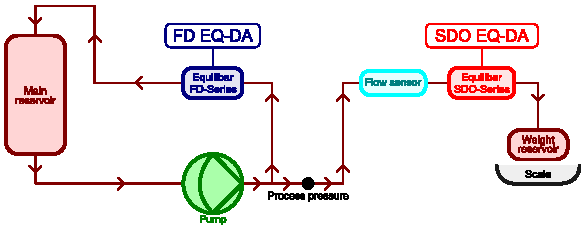
\includegraphics[width=0.8\textwidth]{images/setup.pdf}
    \end{center}
    \vspace{2cm}
    {\Large \CompanyName \par}
    \vspace{0.25cm}
    {\small Author: \AuthorName \par}
    \vspace{0.25cm}
    {\small Report Version: \VersionNumber \par}
    \vspace{0.25cm}
    {\small Date: \ReportDate \par}
    \vfill
\end{titlepage}

\section*{Introduction}
This report presents the results of an experimental evaluation of the shot dosing performance of a Quattroflow QF150 SU pump in combination with an Equilibar SDO backpressure regulator. The experiments were conducted to assess the accuracy and repeatability of the shot dosing process under different pump speeds and control strategies (based on timing and on real-time volume) on Friday, March 13, 2026 and Friday, May 1, 2026. The report is structured as follows: Section \ref{sec:setup} describes the experimental setup, including the components used and their configuration. Section \ref{sec:open_loop} presents the results of open-loop control experiments based on timing, Section \ref{sec:closed_loop} discusses the results of closed-loop control experiments based on real-time integrated volume, and Section \ref{sec:adaptive_closed_loop} discusses the results of an adaptive algorithm that adjusts the closing volume. Finally, Section \ref{sec:conclusion} and \ref{sec:recommendations} provides conclusions and recommendations for future investigations.

\tableofcontents
\newpage

\section{Setup}
\label{sec:setup}
\subsection{Schematic}
Figure \ref{fig:setup} shows a schematic of the experimental setup used to evaluate the shot dosing performance of the Quattroflow QF150 SU pump in combination with an Equilibar SDO backpressure regulator. The main reservoir is filled with water, which is pumped by the Quattroflow pump. The pump is manually controlled and generates a process pressure that depends on the system resistance. Downstream of the pump, an Equilibar FD-series regulator is installed. The reference pressure on this Equilibar ($P_{\text{ref,FD}}$) is controlled by the PCS software, ensuring that the process pressure does not exceed the setpoint. In this way, the pump can operate continuously, while the FD-series Equilibar maintains the desired pressure.

A second Equilibar (SDO-series) is also connected downstream of the pump via a coriolis flow sensor. The output of this regulator is collected in a reservoir mounted on a scale. The reference pressure of the SDO Equilibar ($P_{\text{ref,SDO}}$) is controlled by custom software, such that a specific amount of fluid is collected in the reservoir. Ideally, accurate shot dosing can be achieved by opening the SDO-series Equilibar for a specific duration.

\begin{figure}[!ht]
    \centering
    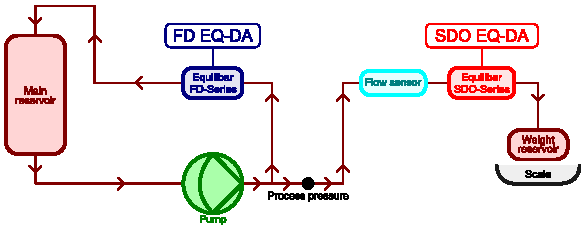
\includegraphics[width=1\textwidth]{images/setup.pdf}
    \caption{Schematic of the experimental setup used to evaluate the shot dosing performance of the Quattroflow QF150 SU pump in combination with an Equilibar SDO backpressure regulator.}
    \label{fig:setup}
\end{figure}

\subsection{Flow sensor}
As a flow sensor, a coriolis SumoFlo 032\footnote{\href{https://www.psgdover.com/biotech/products/coriolis-flow-meters}{https://www.psgdover.com/biotech/products/coriolis-flow-meters}} is used with a maximum flow rate of 3000 ml/min (50 ml/sec). The sensor output is a current signal between 4 and 20 mA, which is converted to a digital signal by the SDO EQ-DA. The flow rate is calculated from the current signal using the following formula:
\begin{equation}
    Q = \frac{I - 4}{16} \cdot 3000,
\end{equation}
where $Q$ is the flow rate in ml/min and $I$ is the current signal in mA. To maximize the bandwidth of the sensor, any onboard filtering (by the SumoFlo) is disabled.

\newpage
\section{Open-loop control}
\label{sec:open_loop}

\subsection{Method}
\label{sec:open_loop_method}
For the open-loop control experiments, the Quattroflow pump is operated at fixed speeds of 250, 500, 750, and 1000 rpm. Since the pump uses a membrane design, the corresponding flow rates are expected to be 300, 600, 900, and 1200 mL/min, respectively.  

During all experiments, the FD-series Equilibar regulator is set to a reference pressure of 1.5 bar ($P_{\mathrm{ref,FD}}=1.5~\mathrm{bar}$), limiting the process pressure to this value while the pump is operating continuously. The SDO-series Equilibar is initially set to a reference pressure of 2 bar, which keeps it fully closed. At each pump speed, the SDO reference pressure $P_{\mathrm{ref,SDO}}$ is allowed to stabilize at 2 bar for 10 seconds before a setpoint of 0 bar is applied for 5 seconds. The process pressure is then increased back to 2 bar. This sequence is referred to as a shot. Four shots are performed at each pump speed. After each shot, the scale reading is recorded and tared to zero before the next shot. During the experiments, data is recorded at a frequency of 1000 Hz, including the reference pressure, the reference setpoint, temperature, valve positions, and flow. The experimental procedure is visualized in the flowchart in Figure \ref{fig:openloop_method}.

\begin{figure}[ht]
\centering
\begin{tikzpicture}[
    node distance=0.35cm,
    every node/.style={font=\scriptsize},
    block/.style={
        draw,
        rounded corners,
        align=center,
        minimum width=4.0cm,
        minimum height=0.75cm,
        inner sep=2pt
    },
    decision/.style={
        draw,
        diamond,
        aspect=2,
        align=center,
        inner sep=1pt
    },
    line/.style={-Latex, thick},
    pump/.style={block, fill=green!20},
    fd/.style={block, fill=blue!20},
    sdo/.style={block, fill=red!20},
    mass/.style={block, fill=black!20}
]

% Nodes
\node[block] (start) {Start Experiment};

\node[fd, below=of start] (fd) {
$P_\mathrm{ref,FD}=1.5~\mathrm{bar}$
};

\node[pump, below=of fd] (pump) {
Quattroflow Pump\\
250/500/750/1000 rpm
};

\node[sdo, below=of pump] (sdoinit) {
$P_\mathrm{ref,SDO}\rightarrow2~\mathrm{bar}$\\
SDO closes
};

\node[block, below=of sdoinit] (stab1) {
Delay 10 s\\
No flow through SDO
};

\node[sdo, below=of stab1] (open) {
$P_\mathrm{ref,SDO}\rightarrow0~\mathrm{bar}$\\
SDO opens
};

\node[block, below=of open] (stab2) {
Delay of 5\\
Flow through SDO
};

\node[sdo, below=of stab2] (close) {
$P_\mathrm{ref,SDO}\rightarrow2~\mathrm{bar}$\\
SDO closes
};

\node[decision, below=0.6cm of close] (shots) {
4 shots\\done?
};

\node[mass, right=2.8cm of shots] (tare) {
Record mass \& tare
};

\node[block, below=0.6cm of shots] (nextspeed) {
Next speed / End
};

% Arrows
\draw[line] (start) -- (fd);
\draw[line] (fd) -- (pump);
\draw[line] (pump) -- (sdoinit);
\draw[line] (sdoinit) -- (stab1);
\draw[line] (stab1) -- (open);
\draw[line] (open) -- (stab2);
\draw[line] (stab2) -- (close);
\draw[line] (close) -- (shots);

\draw[line] (shots) -- node[above] {\scriptsize No} (tare);
\draw[line] (tare) |- (stab1.east);

\draw[line] (shots) -- node[right] {\scriptsize Yes} (nextspeed);

\end{tikzpicture}
\caption{Open-loop experimental procedure. During the experiment, the data is recorded at a frequency of 1000 Hz.}
\label{fig:openloop_method}
\end{figure}

\newpage
\subsection{Results}
\subsubsection{Measurement graphs}
Figure \ref{fig:open_loop_results} shows the results of the open-loop control experiments at a pump speed of 250 rpm. The four shots look fairly similar. The first shot is shown in more detail in figure \ref{fig:shot_1} and all shots at different pump speeds in Figure \ref{fig:all_shots}. The process pressure (orange) follows the reference pressure (gray) closely, with some fluctuations around the setpoint. The valve positions show that both the inlet and outlet valves are fully open during the shot, allowing for maximum flow. The flow rate (third graph) shows a clear increase during the shot, reaching flows around 300 ml/min, which is consistent with the expected flow rate for this pump speed.

\begin{figure}[!ht]
    \centering
    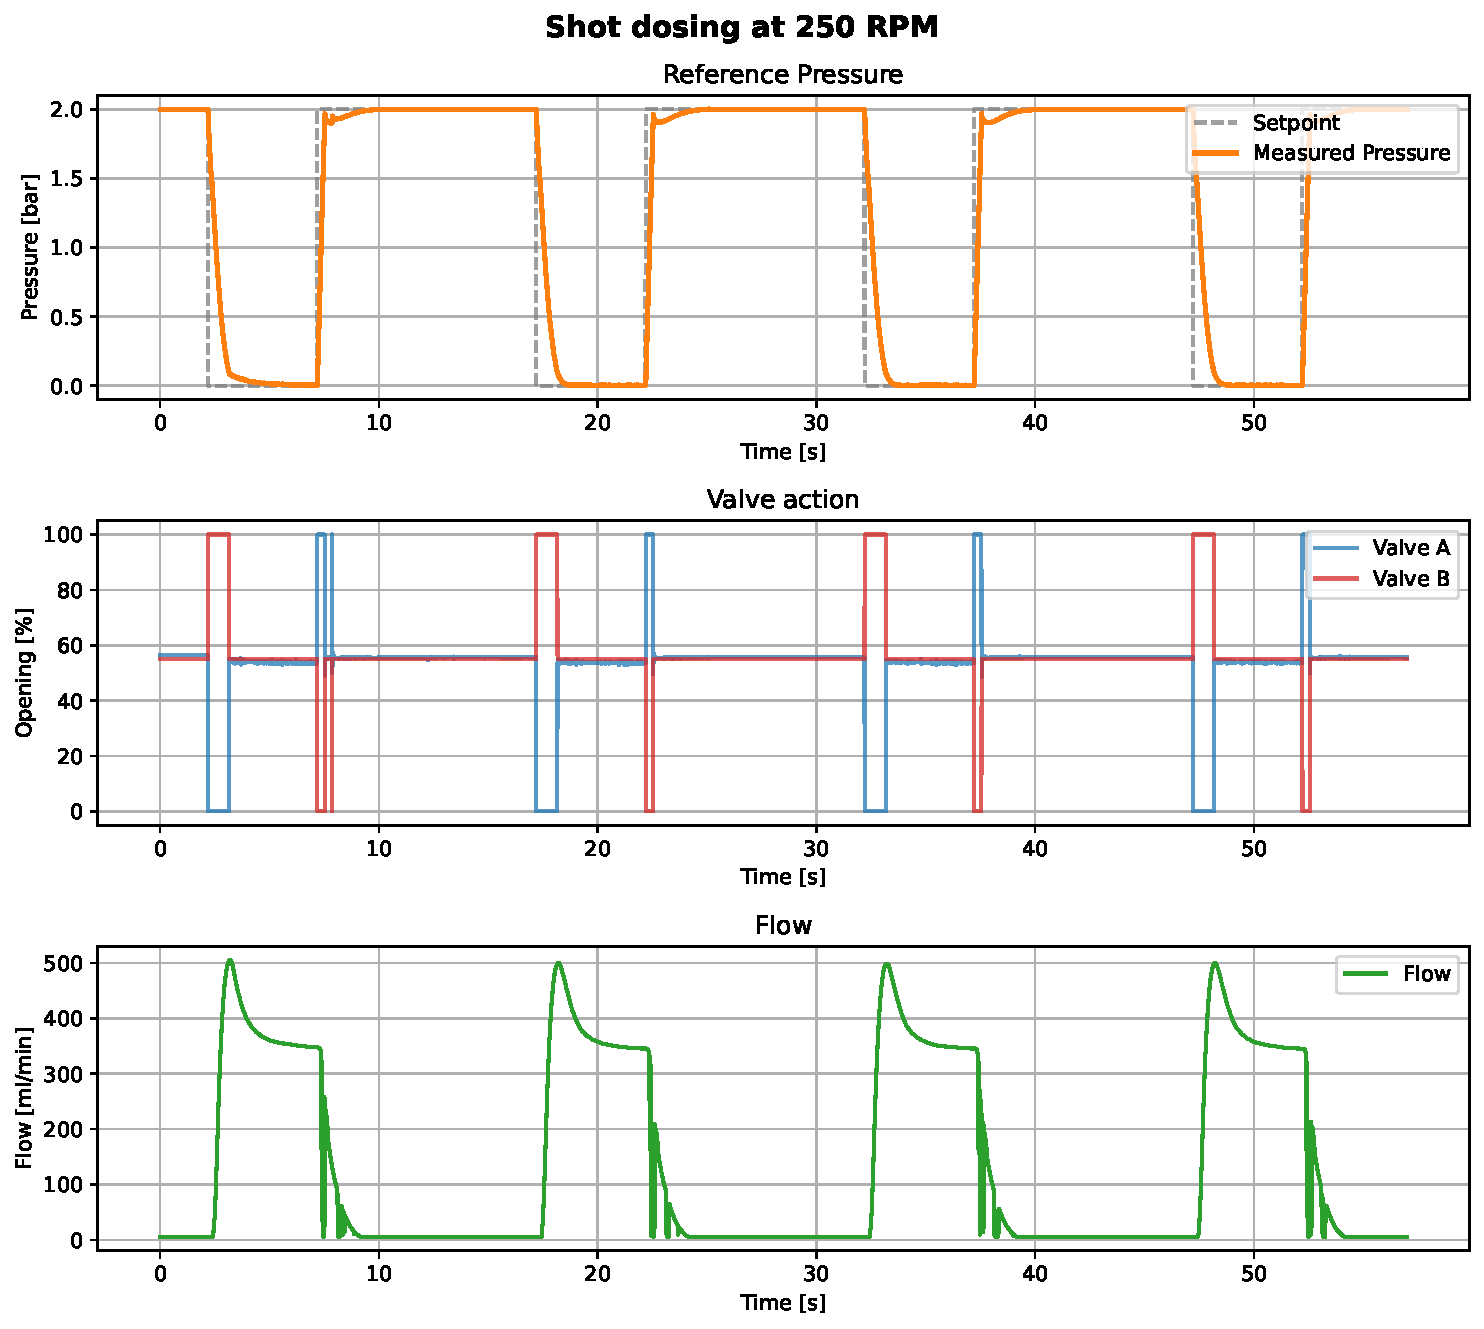
\includegraphics[width=1\textwidth]{images/open_loop_flow_overview_250RPM.pdf}
    \caption{Results of the open-loop control experiments at a pump speed of 250 rpm. The top graph shows the setpoint of the reference pressure on the FD-series Equilibar (gray) and the measured process pressure (orange). The second graph shows the valve positions to create these reference pressures. The in- and outlet valves are fully open to reach the setpoint as fast as possible. The output of the SumoFlo (transformed to ml/min) is shown in the third graph. Four shots are visible.}
    \label{fig:open_loop_results}
\end{figure}

\begin{figure}[!ht]
    \centering
    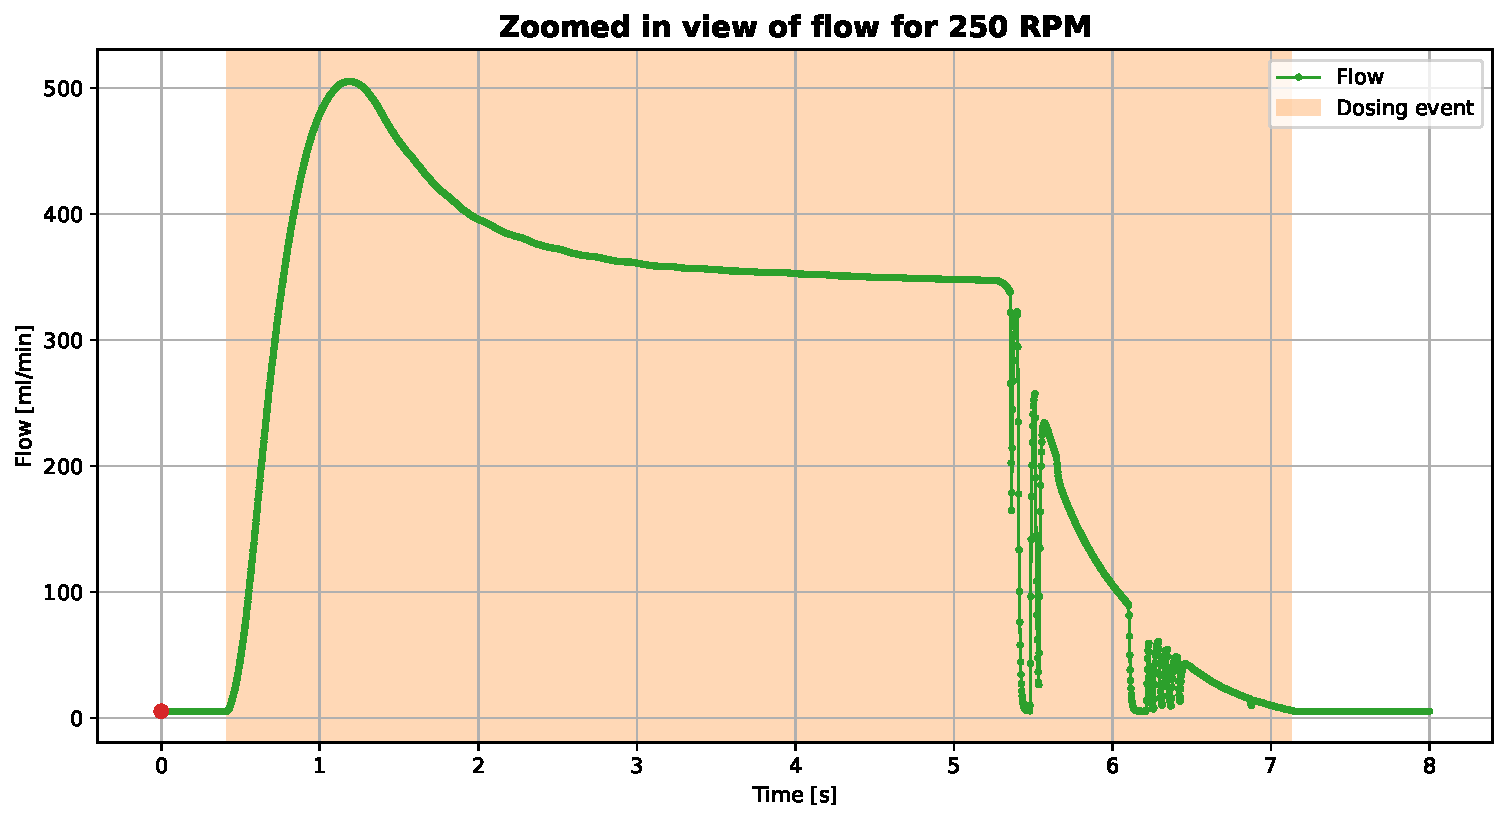
\includegraphics[width=1\textwidth]{images/open_loop_flow_zoomed_250RPM.pdf}
    \caption{Detailed view of the first shot at a pump speed of 250 rpm. The small green dots represent a single measurement point. The sensor gives a positive output flow rate when there is no flow, which is represented by the red dot: it is slightly above 0. The orange area is defined as a dosing event (defined as a flow of $>$ 6 ml/min), which is later used to calculate the amount of fluid dosed during the shot.}
    \label{fig:shot_1}
\end{figure}

\begin{figure}
    \centering
    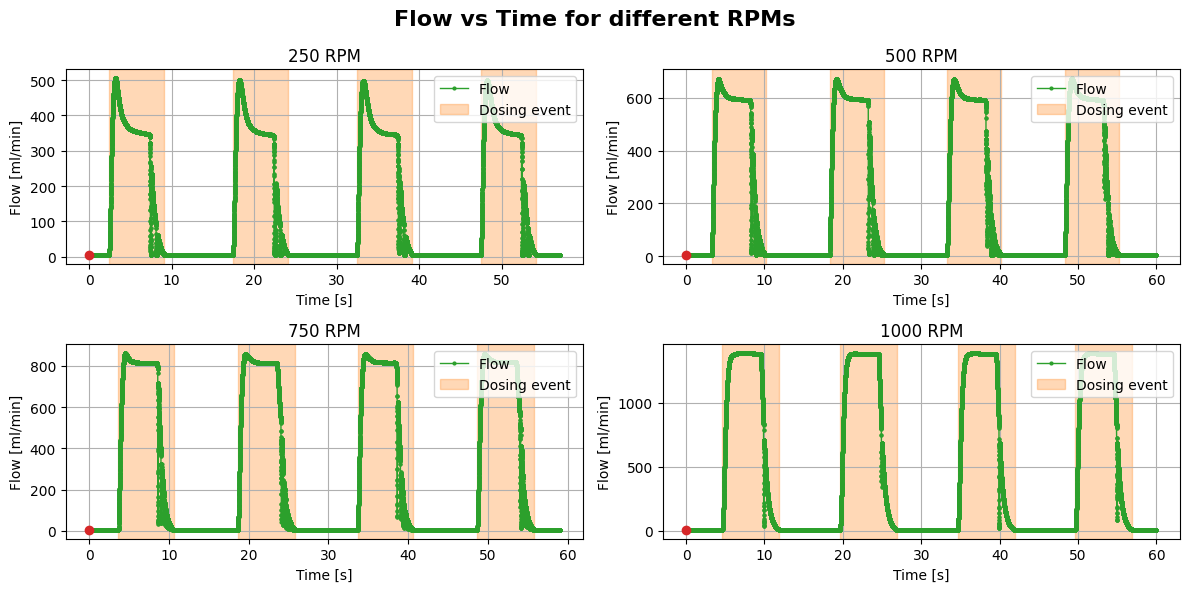
\includegraphics[width=1\textwidth]{images/open_loop_flow_all_cases.png}
    \caption{Results of the open-loop shot dosing control experiments at pump speeds of 250, 500, 750, and 1000 rpm with the Equilibar SDO activated four consecutive times.}
    \label{fig:all_shots}
\end{figure}

\clearpage
\subsubsection{Dose volume calculation}
For every shot, the amount of fluid dosed is calculated by integrating the flow from the SumoFlo sensor ($Q_{\text{SF}}$) over the duration of the shot (the orange area in figure \ref{fig:shot_1}) using: 
\begin{equation}
    V_{\text{SF}} = \sum_{t=t_1}^{t_2} \left[Q_{\text{SF}}(t) - Q_{\text{SF}}(0)\right] \cdot \Delta t,
    \label{eq:sum}
\end{equation}
where $V_{\text{SF}}$ is the volume of fluid dosed in ml determined from the SumoFlo sensor, $Q_{\text{SF}}(t)$ is the flow rate at time $t$ in ml/s from the SumoFlo sensor, $\Delta t$ is the time step, and $Q_{\text{SF}}(0)$ is the initial flow rate (red dots in Figures \ref{fig:shot_1} and \ref{fig:all_shots}), and $t_1$ and $t_2$ are the start and end times of the shot.

\subsubsection{SumoFlo integration vs scale measurements}
Shot volume calculations $V_{\text{SF}}$ and scale measurements $V_{\text{Scale}}$, including the mean and standard deviation (SD), are shown in Table \ref{tab:shot_results_open_loop}.
\begin{table}[!ht]
\centering
\resizebox{\textwidth}{!}{%
\begin{tabular}{c cc cc cc cc cc cc}
\toprule
\multirow{3}{*}{\makecell{\textbf{Pump} \\ \textbf{Speed} \\ (RPM)}}
& \multicolumn{2}{c}{\textbf{Shot 1}}
& \multicolumn{2}{c}{\textbf{Shot 2}}
& \multicolumn{2}{c}{\textbf{Shot 3}}
& \multicolumn{2}{c}{\textbf{Shot 4}}
& \multicolumn{2}{c}{\textbf{Mean}}
& \multicolumn{2}{c}{\textbf{SD}} \\
\cmidrule(lr){2-3} \cmidrule(lr){4-5} \cmidrule(lr){6-7} \cmidrule(lr){8-9} \cmidrule(lr){10-11} \cmidrule(lr){12-13}
& \makecell{\textbf{$V_{\text{SF}}$} \\ (ml)} & \makecell{\textbf{$V_{\text{Scale}}$} \\ (g)}
& \makecell{\textbf{$V_{\text{SF}}$} \\ (ml)} & \makecell{\textbf{$V_{\text{Scale}}$} \\ (g)}
& \makecell{\textbf{$V_{\text{SF}}$} \\ (ml)} & \makecell{\textbf{$V_{\text{Scale}}$} \\ (g)}
& \makecell{\textbf{$V_{\text{SF}}$} \\ (ml)} & \makecell{\textbf{$V_{\text{Scale}}$} \\ (g)}
& \makecell{\textbf{$V_{\text{SF}}$} \\ (ml)} & \makecell{\textbf{$V_{\text{Scale}}$} \\ (g)}
& \makecell{\textbf{$V_{\text{SF}}$} \\ (ml)} & \makecell{\textbf{$V_{\text{Scale}}$} \\ (g)} \\
\midrule
250 & 31.75 & 30 & 31.37 & 30 & 31.46 & 30 & 31.33 & 30 & 31.48 & 30.00 & 0.17 & 0.00 \\
500 & 50.59 & 48 & 50.68 & 48 & 50.26 & 48 & 51.02 & 47 & 50.64 & 47.75 & 0.27 & 0.43 \\
750 & 68.74 & 64 & 70.66 & 64 & 68.17 & 64 & 70.89 & 64 & 69.62 & 64.00 & 1.18 & 0.00 \\
1000 & 115.55 & 105 & 115.75 & 108 & 115.22 & 105 & 115.46 & 106 & 115.50 & 106.00 & 0.19 & 1.22\\
\bottomrule
\end{tabular}
}
\caption{Dosed volumes obtained via SumoFlo integration ($V_{\text{SF}}$) and scale measurements ($V_{\text{Scale}}$) for different pump speeds when the SDO valve is opened for 5 seconds.}
\label{tab:shot_results_open_loop}
\end{table}

\subsubsection{Coefficient of variation}
The coefficient of variation (CV) is calculated as the standard deviation divided by the mean, expressed as a percentage:
\begin{equation}
    \text{CV} = \left( \frac{\sigma}{\mu} \right) \cdot 100\%,
\end{equation}
where $\sigma$ is the standard deviation and $\mu$ is the mean dose volume. The SumoFlo integration values from Table \ref{tab:shot_results_open_loop} are used to create the CV values for SumoFlo integration in Table \ref{tab:cv_open_loop}. The CV values indicate that the repeatability of the dosing process is generally good. However, at 750 RPM, the CV is somewhat increased, indicating more variability in the dosing process at higher speeds. CV calculation for scale measurements is not included as the scale readings do not provide mass measurements in decimals, which is not sufficient to calculate a meaningful CV.

\begin{table}[h!]
\centering
\begin{tabular}{c cc}
\toprule
\textbf{Pump Speed (RPM)} & \textbf{CV (\%)} \\
\midrule
250 & 0.54 \\
500 & 0.53 \\
750 & 1.69 \\
1000 & 0.16 \\
\bottomrule
\end{tabular}
\caption{Coefficient of variation (CV) for the SumoFlo integration dosed volumes ($V_{\text{SF}}$) at different pump speeds.}
\label{tab:cv_open_loop}
\end{table}

\newpage

\subsubsection{Error analysis}
The volume calculations allow a comparison of the SumoFlo integration volume with the scale measurements. The percentage error of the SumoFlo integration relative to the scale measurements is calculated using the following formula:
\begin{equation}
    \text{Percentage Error} = \left| \frac{V_{\text{SF}} - V_{\text{Scale}}}{V_{\text{Scale}}} \right| \cdot 100\%,
\end{equation}
where $V_{\text{SF}}$ is the volume calculated from the SumoFlo sensor fusion and $V_{\text{Scale}}$ is the volume measured by the scale. These results are shown in Table \ref{tab:percentage_error}. The color coding in the table indicates the magnitude of the percentage error: green for 0–5\%, yellow for 5–10\%, and orange for above 10\%. From the results, it is clear that at all speeds the SumoFlo integration overestimates the dosed volume compared to the scale measurements, and that at higher pump speeds the percentage error increases significantly. An overestimation can be caused by calibration issues, but then a constant percentage of overshoot is expected. An increasing percentage error at higher pump speeds could indicate that the closing behavior of the SDO-series Equilibar is different at higher flow rates, e.g., slower which causes a larger overshoot at higher flow rates.

\begin{table}[!ht]
\centering
\begin{tabular}{c cccc}
\toprule
\makecell{\textbf{Pump Speed} (RPM)}
& \textbf{Shot 1 (\%)}
& \textbf{Shot 2 (\%)}
& \textbf{Shot 3 (\%)}
& \textbf{Shot 4 (\%)} \\
\midrule
250 & \cellcolor{yellow!25}5.84 & \cellcolor{green!15}4.56 & \cellcolor{green!15}4.87 & \cellcolor{green!15}4.43 \\
500 & \cellcolor{yellow!25}5.39 & \cellcolor{yellow!25}5.58 & \cellcolor{green!15}4.71 & \cellcolor{yellow!25}8.56 \\
750 & \cellcolor{yellow!25}7.41 & \cellcolor{orange!30}10.40 & \cellcolor{yellow!25}6.52 & \cellcolor{orange!30}10.77 \\
1000 & \cellcolor{orange!30}10.05 & \cellcolor{yellow!25}7.18 & \cellcolor{yellow!25}9.73 & \cellcolor{yellow!25}8.92 \\
\bottomrule
\end{tabular}
\caption{Percentage error of the SumoFlo integration volume ($V_{\text{SF}}$) relative to scale measurements ($V_{\text{Scale}}$) for different pump speeds. Color indicates error magnitude.}
\label{tab:percentage_error}
\end{table}

\clearpage
\section{Closed-loop control}
\label{sec:closed_loop}
In the open-loop experiments, the shot dosing was performed without real-time feedback and just timing based. Based on these results, a closed-loop control experiment is set up to control the reference pressure of the SDO-series Equilibar ($P_{\text{ref,SDO}}$) in real-time based on a real-time integration using the SumoFlo sensor. Ideally, a shot dosing $V_{\text{Target}}$ can be defined, independent of a pump speed.

\subsection{Method}
\label{sec:closed_loop_method}
Method from Section \ref{sec:open_loop_method} is used, but now $P_{\text{ref,SDO}}$ is controlled by custom software to achieve a specific dose volume $V_{\text{Target}}$. The SumoFlo sensor integration is performed in real-time, and the reference pressure of the SDO-series Equilibar is set to 2 bar when the target volume is reached, which closes the SDO valve and stops the flow. Again, four shots are performed at each pump speed of 250, 500, 750, and 1000 rpm. $V_{\text{Target}}$ is set to 50 ml. The experimental procedure is visualized in the flowchart in Figure \ref{fig:closed_loop_method}.

\begin{figure}[ht]
\centering
\begin{tikzpicture}[
    node distance=0.35cm,
    every node/.style={font=\scriptsize},
    block/.style={
        draw,
        rounded corners,
        align=center,
        minimum width=4.3cm,
        minimum height=0.75cm,
        inner sep=2pt
    },
    decision/.style={
        draw,
        diamond,
        aspect=2,
        align=center,
        inner sep=1pt
    },
    decision1/.style={
        draw,
        diamond,
        aspect=2,
        align=center,
        inner sep=1pt,
        fill=cyan!20
    },
    line/.style={-Latex, thick},
    pump/.style={block, fill=green!20},
    fd/.style={block, fill=blue!20},
    sdo/.style={block, fill=red!20},
    mass/.style={block, fill=black!20},
    flow/.style={block, fill=orange!20},
    sensor/.style={block, fill=cyan!20}
]

% Nodes
\node[block] (start) {Start Experiment};

\node[fd, below=of start] (fd) {
$P_\mathrm{ref,FD}=1.5~\mathrm{bar}$
};

\node[pump, below=of fd] (pump) {
Quattroflow Pump\\
250/500/750/1000 rpm
};

\node[sdo, below=of pump] (sdoinit) {
$P_\mathrm{ref,SDO}\rightarrow2~\mathrm{bar}$\\
SDO closes
};

\node[block, below=of sdoinit] (stab1) {
Delay 10 s\\
No flow through SDO
};

\node[sdo, below=of stab1] (open) {
$P_\mathrm{ref,SDO}\rightarrow0~\mathrm{bar}$\\
SDO opens
};

\node[sensor, below=of open] (integration) {
Real-time SumoFlo integration\\
$V_{\text{Target}} = 50$ ml
};

\node[decision1, below=0.6cm of integration] (target) {
$V_{\text{Target}}$\\
reached?
};

\node[sdo, below=0.6cm of target] (close) {
$P_\mathrm{ref,SDO}\rightarrow2~\mathrm{bar}$\\
SDO closes
};

\node[decision, below=0.6cm of close] (shots) {
4 shots\\
done?
};

\node[mass, right=3.2cm of shots] (tare) {
Record mass \& tare
};

\node[block, below=0.6cm of shots] (nextspeed) {
Next speed / End
};

% Arrows
\draw[line] (start) -- (fd);
\draw[line] (fd) -- (pump);
\draw[line] (pump) -- (sdoinit);
\draw[line] (sdoinit) -- (stab1);
\draw[line] (stab1) -- (open);
\draw[line] (open) -- (integration);
\draw[line] (integration) -- (target);

\draw[line] (target) -- node[right] {\scriptsize Yes} (close);
\draw[line] (target.east) -- ++(1.5,0) |- node[pos=0.25,right] {\scriptsize No} (integration.east);

\draw[line] (close) -- (shots);

\draw[line] (shots) -- node[above] {\scriptsize No} (tare);
\draw[line] (tare) |- (stab1.east);

\draw[line] (shots) -- node[right] {\scriptsize Yes} (nextspeed);

\end{tikzpicture}
\caption{Closed-loop experimental procedure. During the experiment, the data is recorded at a frequency of 1000 Hz.}
\label{fig:closed_loop_method}
\end{figure}

\newpage
\subsection{Results}
\subsubsection{Measurement graphs}
The raw measurement graphs look very similar to the open-loop control experiments, but now $P_{\text{ref,SDO}}$ is increased to 2 bar at the moment $V_{\text{Target}}$ is reached. As this happens within fractions of a second, the difference is hard to see in the graphs. 

\subsubsection{SumoFlo integration vs scale measurements}
More interesting is to look at the dose volumes. The results are shown in Table \ref{tab:closed_loop_results}. Although the target volume was set to 50 ml, the actual dosed volumes are larger. This could be caused by a delay in the closing of the SDO-series Equilibar, which leads to an overshoot in the dosed volume. In the next section an algorithm is implemented to adjust the closing volume of the SDO-series Equilibar based on the previously dosed shot volumes, which is expected to further reduce the percentage error.

\begin{table}[!ht]
\centering
\resizebox{\textwidth}{!}{%
\begin{tabular}{c cc cc cc cc cc cc}
\toprule
\multirow{3}{*}{\makecell{\textbf{Pump} \\ \textbf{Speed} \\ (RPM)}}
& \multicolumn{2}{c}{\textbf{Shot 1}}
& \multicolumn{2}{c}{\textbf{Shot 2}}
& \multicolumn{2}{c}{\textbf{Shot 3}}
& \multicolumn{2}{c}{\textbf{Shot 4}}
& \multicolumn{2}{c}{\textbf{Mean}}
& \multicolumn{2}{c}{\textbf{SD}} \\
\cmidrule(lr){2-3} \cmidrule(lr){4-5} \cmidrule(lr){6-7} \cmidrule(lr){8-9} \cmidrule(lr){10-11} \cmidrule(lr){12-13}
& \makecell{\textbf{$V_{\text{SF}}$} \\ (ml)} & \makecell{\textbf{$V_{\text{Scale}}$} \\ (g)}
& \makecell{\textbf{$V_{\text{SF}}$} \\ (ml)} & \makecell{\textbf{$V_{\text{Scale}}$} \\ (g)}
& \makecell{\textbf{$V_{\text{SF}}$} \\ (ml)} & \makecell{\textbf{$V_{\text{Scale}}$} \\ (g)}
& \makecell{\textbf{$V_{\text{SF}}$} \\ (ml)} & \makecell{\textbf{$V_{\text{Scale}}$} \\ (g)}
& \makecell{\textbf{$V_{\text{SF}}$} \\ (ml)} & \makecell{\textbf{$V_{\text{Scale}}$} \\ (g)}
& \makecell{\textbf{$V_{\text{SF}}$} \\ (ml)} & \makecell{\textbf{$V_{\text{Scale}}$} \\ (g)} \\
\midrule
250 & 51.59 & 50 & 51.47 & 50 & 51.49 & 50 & 51.41 & 51 & 51.49 & 50.25 & 0.07 & 0.43 \\
500 & 54.90 & 52 & 55.23 & 52 & 55.19 & 52 & 55.73 & 52 & 55.26 & 52.00 & 0.30 & 0.00 \\
750 & 58.41 & 54 & 58.18 & 55 & 57.64 & 54 & 60.06 & 55 & 58.57 & 54.50 & 0.90 & 0.50 \\
1000 & 59.97 & 55 & 59.85 & 56 & 60.06 & 55 & 59.84 & 56 & 59.93 & 55.50 & 0.09 & 0.50 \\
\bottomrule
\end{tabular}
}
\caption{Dosed volumes obtained via SumoFlo integration ($V_{\text{SF}}$) and scale measurements ($V_{\text{Scale}}$) for different pump speeds. $V_{\text{Target}}$ was set to 50 ml.}
\label{tab:closed_loop_results}
\end{table}

\subsubsection{Coefficient of variation}
Again, the coefficient of variation (CV) is calculated as the standard deviation divided by the mean, expressed as a percentage. The SumoFlo integration values from Table \ref{tab:closed_loop_results} are used to create the CV values for SumoFlo integration in Table \ref{tab:cv_closed_loop}. The CV values indicate that the repeatability of the dosing process is generally good, and is similar to the open-loop control experiments. Still, an increase in CV is observed at 750 RPM, which could indicate that at this speed the corriodis sensor is less accurate.
\begin{table}[h!]
\centering
\begin{tabular}{c cc}
\toprule
\textbf{Pump Speed (RPM)} & \textbf{CV (\%)} \\
\midrule
250 & 0.14 \\
500 & 0.54 \\
750 & 1.54 \\
1000 & 0.15 \\
\bottomrule
\end{tabular}
\caption{Coefficient of variation (CV) for the SumoFlo integration dosed volumes ($V_{\text{SF}}$) at different pump speeds for the closed-loop control experiments.}
\label{tab:cv_closed_loop}
\end{table}

% \begin{table}[!ht]
% \centering
% \begin{tabular}{c cccc}
% \toprule
% \makecell{\textbf{Pump Speed} (RPM)}
% & \textbf{Shot 1 (\%)}
% & \textbf{Shot 2 (\%)}
% & \textbf{Shot 3 (\%)}
% & \textbf{Shot 4 (\%)} \\
% \midrule
% 250 & \cellcolor{green!15}3.18 & \cellcolor{green!15}2.94 & \cellcolor{green!15}2.98 & \cellcolor{green!15}2.82 \\
% 500 & \cellcolor{yellow!25}5.58 & \cellcolor{yellow!25}6.21 & \cellcolor{yellow!25}6.13 & \cellcolor{yellow!25}7.17 \\
% 750 & \cellcolor{yellow!25}6.20 & \cellcolor{yellow!25}5.78 & \cellcolor{green!15}4.80 & \cellcolor{yellow!25}7.25 \\
% 1000 & \cellcolor{yellow!25}9.04 & \cellcolor{yellow!25}8.82 & \cellcolor{yellow!25}9.20 & \cellcolor{yellow!25}8.80 \\
% \bottomrule
% \end{tabular}
% \caption{Percentage error of the SumoFlo integration volume ($V_{\text{SF}}$) relative to scale measurements ($V_{\text{Scale}}$) for different pump speeds. Color indicates error magnitude.}
% \label{tab:closed_loop_percentage_error}
% \end{table}



\clearpage
\newpage
\section{Adaptive closed-loop control}
\label{sec:adaptive_closed_loop}
Based on the open-loop and semi-closed-loop control experiements, an adaptive closed-loop control experiment is set up to evaluate whether the accuracy of the shot dosing can be futher improved by timing the closing of the SDO-series Equilibar (by increasing the reference pressure) in real-time based on the \textbf{flow measurements} from the SumoFlo sensor, and \textbf{previous shot dosing volumes}. 

\subsection{Method}
\label{sec:adaptive_closed_loop_method}
Closing the SDO-series Equilibar immediately when the target volume $V_{Target}$ is reached leads to an overshoot in the dosed volume, particularly at higher pump speeds. Increasing the reference pressure and subsequently closing the valve requires a finite amount of time, during which flow continues. To mitigate this effect, the closing volume $V_{Close}$ of the SDO-series Equilibar is adjusted based on the dosing volumes of the previous shots. \\
A simple algorithm is implemented to determine a closing volume $V_{Close}$, at which the reference pressure of the SDO-series Equilibar is increased and the valve starts closing. Since flow continues during the valve closing process, it follows that $V_{Close} < V_{Target}$. After each shot, the closing volume is updated based on the previously dosed shot volume ($V_{SF}$) determined by integrating the flow from the SumoFlo sensor, and the target volume ($V_{Target}$) using the following formula:

\begin{equation}
    V_{Close}(i+1) = V_{Close}(i) \left[ \alpha + \left( 1 - \alpha \right) \frac{V_{Target}}{V_{SF}(i)} \right],\label{eq:adaptive_closed_loop_adjustment}
\end{equation}
where $i$ is the shot number and $\alpha$ is a tuning parameter between 0 and 1 that determines how much the closing volume is adjusted based on the previously dosed shot. For example, if $\alpha$ is set to 0.5, the closing volume will be adjusted halfway towards the target volume based on the previous shot's performance. When $\alpha=0$, this leads to a fast and aggressive adjustment, while $\alpha=1$ leads to no adjustment. The initial closing volume is set to 50 ml, which is equal to the target volume of 50 ml. For our experiments, $\alpha=0$, and eight pulses are performed at each pump speed of 250, 500, 750, and 1000 rpm. 

\begin{figure}[h!]
\centering
\begin{tikzpicture}[
    node distance=0.38cm,
    every node/.style={font=\scriptsize},
    block/.style={
        draw,
        rounded corners,
        align=center,
        minimum width=4.6cm,
        minimum height=0.78cm,
        inner sep=2pt
    },
    decision/.style={
        draw,
        diamond,
        aspect=2,
        align=center,
        inner sep=1pt
    },
    decision1/.style={
        draw,
        diamond,
        aspect=2,
        align=center,
        inner sep=1pt,
        fill=cyan!20
    },
    line/.style={-Latex, thick},
    pump/.style={block, fill=green!20},
    fd/.style={block, fill=blue!20},
    sdo/.style={block, fill=red!20},
    mass/.style={block, fill=black!15},
    flow/.style={block, fill=orange!20},
    sensor/.style={block, fill=cyan!20},
    calc/.style={block, fill=yellow!25}
]

% Nodes
\node[block] (start) {Start Experiment};

\node[fd, below=of start] (fd) {
$P_{\mathrm{ref,FD}} = 1.5~\mathrm{bar}$
};

\node[pump, below=of fd] (pump) {
Quattroflow Pump\\
250 / 500 / 750 / 1000 rpm
};

\node[sdo, below=of pump] (sdoinit) {
Initialize SDO\\
$P_{\mathrm{ref,SDO}} \rightarrow 2~\mathrm{bar}$
};

\node[block, below=of sdoinit] (stab1) {
Delay 10 s\\
No flow through SDO
};

\node[calc, below=of stab1] (vclose) {
Set current closing volume\\
$V_{\mathrm{Close}}(i)$
};

\node[sdo, below=of vclose] (open) {
Open SDO\\
$P_{\mathrm{ref,SDO}} \rightarrow 0~\mathrm{bar}$
};

\node[sensor, below=of open] (integration) {
Real-time SumoFlo integration\\
Measure $V_{\mathrm{SF}}$
};

\node[decision1, below=0.7cm of integration] (closecond) {
$V_{\mathrm{SF}} \geq V_{\mathrm{Close}}$?
};

\node[sdo, below=0.7cm of closecond] (close) {
Close SDO\\
$P_{\mathrm{ref,SDO}} \rightarrow 2~\mathrm{bar}$
};

\node[sensor, below=of close] (integration2) {
Real-time SumoFlo integration\\
Measure $V_{\mathrm{SF}}$
};

\node[decision1, below=0.7cm of integration2] (closecond2) {
5 s after closing?
};

\node[calc, below=0.7cm of closecond2] (update) {
Update closing volume\\
$\displaystyle
V_{\mathrm{Close}}(i+1)\approx
V_{\mathrm{Close}}(i)
\frac{V_{\mathrm{Target}}}{V_{\mathrm{SF}}(i)}
$
};

\node[decision, below=0.8cm of update] (shots) {
8 shots\\
completed?
};


\node[mass, right=3.4cm of shots] (record) {
Record mass \& tare
};

    
\node[block, below=0.8cm of shots] (nextspeed) {
Next speed / End experiment
};

% Arrows
\draw[line] (start) -- (fd);
\draw[line] (fd) -- (pump);
\draw[line] (pump) -- (sdoinit);
\draw[line] (sdoinit) -- (stab1);
\draw[line] (stab1) -- (vclose);
\draw[line] (vclose) -- (open);
\draw[line] (open) -- (integration);
\draw[line] (integration) -- (closecond);

\draw[line] (closecond) -- node[right] {\scriptsize Yes} (close);

\draw[line] (closecond.east) -- ++(1.6,0)
    |- node[pos=0.25,right] {\scriptsize No}
    (integration.east);

\draw[line] (close) -- (integration2);
\draw[line] (integration2) -- (closecond2);

\draw[line] (closecond2) -- node[right] {\scriptsize Yes} (update);

\draw[line] (closecond2.east) -- ++(1.6,0)
    |- node[pos=0.25,right] {\scriptsize No}
    (integration2.east);

\draw[line] (shots) -- node[above] {\scriptsize No} (record);

\draw[line] (record) |- (vclose.east);

% \draw[line] (update.west) -| (stab1.west);
\draw[line] (update) -- (shots);

\draw[line] (shots) -- node[right] {\scriptsize Yes} (nextspeed);

\end{tikzpicture}

\caption{
Adaptive closed-loop dosing procedure. The SumoFlo sensor signal is integrated in real time to determine the dispensed volume. The SDO-series Equilibar closes once the measured volume reaches the adaptive closing volume $V_{\mathrm{Close}}$. After each shot, $V_{\mathrm{Close}}$ is updated using the measured shot volume to compensate for valve closing delay and reduce dosing overshoot. Data is recorded at 1000 Hz.
}
\label{fig:adaptive_closed_loop_method}
\end{figure}

\subsubsection{Calibration}
Before performing the adaptive closed-loop control experiments, the SumoFlo sensor is calibrated to ensure that the flow measurements are accurate. As there was no other flow sensor in the setup, the calibration is performed by comparing the integrated volume from the SumoFlo sensor measurements with the scale measurements. The SDO-series Equilibar is opened for fixed amounts of time and the flow measurments are scaled such that the integrated volume matches the scale measurements. A different option to calibrate the flow sensor was to use the membrane pump output flow, however, this method was not used.

\clearpage
\newpage
\subsection{Results}
The results of the adaptive closed-loop control experiments are shown in Figure \ref{fig:adaptive_closed_loop_shots}. The results indicate that at lower pump speeds, the shots volumes converge within a single shot towards the target volume, while at higher pump speeds, it takes three shots to converge towards the target volume. This results are for the most aggressive setting of $\alpha=0$. For higher values of $\alpha$, it takes more shots to converge towards the target volume, but any fluctiations in the flow measurements will have less impact on the closing volume, which may lead to more stable results.

\begin{figure}[h!]
    \centering
    \includegraphics[width=1\textwidth]{images/closed_loop_control_shots.pdf}
    \caption{Comparison between the target volume $V_{Target}$ (gray), the volume calculated from the SumoFlo sensor $V_{SF}$ (red), and the scale measurements $V_{Scale}$ (blue bars) for different pump speeds while $\alpha=0$ in Equation \ref{eq:adaptive_closed_loop_adjustment}. As the scale generates non-decimal values, a bar is plotted for $V_{Scale}$ from $V_{Scale}-0.5g$ to $V_{Scale}+0.5g$ to give a better visual representation of the results.}
    \label{fig:adaptive_closed_loop_shots}
\end{figure}
\clearpage
\newpage
\section{Conclusion}
\label{sec:conclusion}
\begin{itemize}
    \item The open-loop control experiments showed that the shot dosing performance of the Quattroflow QF150 SU pump in combination with an Equilibar SDO backpressure regulator shows a reasonably low coefficient of variation (CV) at 250, 500 and 1000 rpm. At 750 rpm, the CV is slightly higher. This could be due to the working frequency of the corriodis sensor.
    \item The closed-loop strategy, where the reference pressure of the SDO-series Equilibar is adjusted in real-time based on flow measurements, creates the opportunity to give a specific target volume and to stop the flow immediately when this target is reached. However, with the current algorithm, overshoots of almost 20\% are observed at higher pump speeds. The latter was caused by the closing behavior of the SDO-series Equilibar, which does not closes instanly after increasing the reference pressure, leading to an overshoot in the dosed volume.
    \item The adaptive closed-loop strategy results in an improvement in shot dosing performance, especially when dealing with different types of pump speeds. The generates volumes always converge towards the target volume, without manual adjustment of the closing volume. However, fluctuating pump speeds during dosing events may lead to fluctuating flow measurements, which may cause the closing volume to fluctuate as well, leading to less stable results. This is especially the case when multiple dosing setups are running in parallel, downstream of a single pump running at a constant speed. Therefore, it is recommended to keep the upstream pressure constant. The latter can be achieved by using a (EQ-DA?) pressure regulator setup upstream of the dosing setup(s).
    \item The closing behavior of the SDO-series Equilibar causes fast fluctuations in the flow rate, which may lead to inaccurate volume measurements by the SumoFlo sensor and could cause deviations in the integration to calculate the dosed volume. 
\end{itemize}

\clearpage
\section{Recommendations for future investigation}
\label{sec:recommendations}
\begin{itemize}
    \item Include a scale that measures the dose volume with digits after the decimal point, which allows for a more accurate measurement of the dosed volume and thus a more accurate calculation of the percentage error.
    \item Calibrate the SumoFlo sensor to ensure that the flow measurements are accurate and that the sensor gives a zero output when there is no flow, and correct increase linearly with flow rate. This may reduce the percentage error and improve the performance of the adaptive closed-loop control strategy.
    \item Investigate if the integration of a pulsed flow through the SumoFlo sensor is correct and whether the fluctuations in the flow rate caused by the SDO-series Equilibar closing are affecting the accuracy of the volume calculations. The results from Figure \ref{fig:adaptive_closed_loop_shots} show that sometimes the SumoFlo sensor integration volumes are different than the scale measurements, which could be caused by inaccurate flow measurements during the closing of the SDO-series Equilibar (or a bad scale).
    \item Investiage if other (cheap) flow sensors can be used to measure the flow rate. Potentially sensors that are able to capture the flow fluctuations more accurately, and not specifically absolute flow rates, which may lead to more accurate volume calculations and better performance of the closed-loop control strategies. Doppler flow sensors could be an interesting option to investigate, as they are able to measure flow rates in real time, and could be connected 'non-intrusively' to the tubing, which may be more suitable for pharmaceutical applications. Calibration of these sensors can be done by looking at the dosed volume instead of the flow rate, which may be more accurate and easier to perform.
\end{itemize}

\newpage
\section*{Version control}
\addcontentsline{toc}{section}{Version control}

\begin{tabular}{|c|c|c|}
\hline
Version & Date & Description \\
\hline
1.0 & March 20, 2026 & Initial draft \\
\hline
1.1 & April 17, 2026 & Corrected wrong values in Table \ref{tab:closed_loop_results} \\
\hline 
1.2 & May 8, 2026 & Included closed-loop results in Section \ref{sec:closed_loop} \\
\hline
1.3 & May 22, 2026 & \makecell{Included adaptive closed-loop results and finished\\report and layout, include method flow diagrams} \\
\hline
\end{tabular}

\end{document}